\section{Considerações Iniciais}

Nos Capítulo~\ref{chapter:catalogo_refactoring_KDM} e~\ref{chapter:Toward_a_Refactoring_Metamodel_for_KDM}, são apresentadas soluções para auxiliar o engenheiro de modernização a aplicar e reutilizar refatorações no contexto da abordagem ADM e do metamodelo KDM. Além disso, no Capítulo~\ref{chapter:ferramenta_kdm_re}, a ferramenta KDM-RE é apresentada. KDM-RE automatiza todo o processo de aplicação, reutilização e propagação de mudanças no contexto do metamodelo KDM, deixando somente sob responsabilidade do engenheiro de software a identificação de onde aplicar refatorações. Desse modo, com o uso dessa ferramenta, o engenheiro de software tem um ambiente de desenvolvimento integrado ao Eclipse, onde refatorações podem ser aplicadas e reutilizadas sem se preocupar com a propagação de mudanças para outras visões/artefatos representadas em uma determinada instância do metamodelo KDM.

Com o objetivo de verificar se as refatorações criadas para o metamodelo KDM realmente melhoraram a qualidade de um sistema, foi realizado um experimento ao longo desta tese. Esse experimento foi planejado e executado seguindo a abordagem definida por~\citeonline{Wohlin}, que é composta por três principais fases: (\textit{i}) definição e planejamento, por meio da qual são especificados o contexto, as hipóteses, as variáveis, os participantes (quando necessário), os instrumentos e o modelo do experimento; (\textit{ii}) operação, na qual ocorre a preparação e a execução do experimento com ou sem os participantes; e (\textit{iii}) análise dos dados, em que os dados coletados durante o experimento são agrupados e analisados por meio de técnicas estatísticas.


%Com o objetivo de verificar se as refatorações criadas para o metamodelo KDM realmente melhoraram a qualidade de um sistema e com o intuito de verificar se a ferramenta KDM-RE proporciona facilidade e eficiência na prática, foram realizados dois experimentos ao longo desta tese. Esses experimentos foram planejados e executados seguindo a abordagem definida por~\citeonline{Wohlin}, que é composta por três principais fases: (\textit{i}) definição e planejamento, por meio da qual são especificados o contexto, as hipóteses, as variáveis, os participantes (quando necessário), os instrumentos e o modelo do experimento; (\textit{ii}) operação, na qual ocorre a preparação e a execução do experimento com ou sem os participantes; e (\textit{iii}) análise dos dados, em que os dados coletados durante o experimento são agrupados e analisados por meio de técnicas estatísticas.

Na Seção~\ref{sec:teste_estatisticos}, há uma descrição dos testes estatísticos aplicados no experimento realizado. Na Seção~\ref{sec:experimento}, é descrito o experimento que verifica se as refatorações criadas para o metamodelo KDM realmente melhoram a qualidade de um sistema. Em seguida, na Seção~\ref{sec:consideracoes_finais_experimento}, são comentadas as considerações finais deste capítulo.

%Na Seção~\ref{sec:teste_estatisticos}, há uma descrição dos testes estatísticos aplicados no experimento realizado. Na Seção~\ref{sec:experimento}, é descrito o experimento que verifica se as refatorações criadas para o metamodelo KDM realmente melhoram a qualidade de um sistema. Na Seção~\ref{sec:experimento_KDM_re}, é apresentado um experimento que avaliou a ferramenta KDM-RE\unsure{ver}. Em seguida, na Seção~\ref{sec:consideracoes_finais_experimento}, são comentadas as considerações finais deste capítulo.

\section{Testes Estatísticos}\label{sec:teste_estatisticos}

~\citeonline{Wohlin} declaram que os experimentos almejam responder questões a respeito de um objeto de estudo. Para cada questão, são definidas uma ou mais métricas a partir da(s) qual(is) os dados são coletados e, também, um conjunto de hipóteses sobre os possíveis resultados é definido. Esse conjunto de hipóteses é formado por:

\begin{itemize}
\item Uma \textbf{hipótese nula}: Considera que não há uma diferença significativa entre os dados obtidos ao se aplicarem os diferentes tratamentos sobre o objeto de estudo;
\item Uma ou mais \textbf{hipóteses alternativas}: Considera(m) os demais possíveis resultados. Por exemplo, a hipótese alternativa 1 considera que a ferramenta X é mais eficiente do que a ferramenta Y, e a hipótese alternativa 2 considerada que a ferramenta X é menos eficiente do que a ferramenta Y.
\end{itemize}

Alguns cálculos podem ser realizados sobre os dados coletados para obter um resultado e uma das hipóteses alternativas ser aceita. Por exemplo, cálculos de média e de porcentagem podem indicar que, em determinado experimento, o tempo gasto pelos participantes para aplicar refatorações no metamodelo KDM foi menor quando a ferramenta X foi utilizada do que quando a ferramenta Y foi utiliza. Contudo, ainda se fazem necessários testes estatísticos para comprovar que esse resultado é significativo, refutando-se, assim, a hipótese nula.

No experimento apresentado nesta tese, foram aplicados os testes estatísticos \textbf{Shapiro-Wilk} e \textbf{Paried T-Test}, com o apoio da ferramenta R\footnote{\texttt{https://www.r-project.org/}}. Esses testes são brevemente explicados a seguir.% \change{mudar Colocar os testes estatisticos realmentes utilizados}

\begin{figure}[h]
	\centering
	\caption{Representação gráfica de uma distribuição normal de dados.}
	\label{fig:shapiro_wilk}
	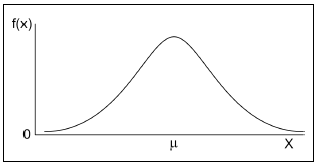
\includegraphics[scale=0.9]{images/distribuicao_normal}
	\fautor
\end{figure}

\subsection{Shapiro-Wilk e Paired T-Test}\label{sec:shapiro_wilk}

O teste \textbf{Shapiro-Wilk} é aplicado para verificar se um conjunto de dados segue, ou não, uma distribuição normal, que possui graficamente o formato de um sino simétrico em relação à sua média (ver Figura~\ref{fig:shapiro_wilk}). Se o p-valor (resultado) do teste \textbf{Shapiro-Wilk} sobre um conjunto de dados for menor do que 0.05, significa que a chance dos dados seguirem uma distribuição normal é menor do que 5\%. Quando esse resultado ocorre, considera-se, estatisticamente, que os dados não seguem uma distribuição normal~\cite{Wohlin}. 


Em geral, as ferramentas de estatísticas utilizam um gráfico de probabilidade, também conhecido como \textit{Q-Q Plot}, para representar graficamente a distribuição de um conjunto de dados. Nesse gráfico, quando os dados se posicionam ao redor da linha diagonal, considera-se que eles seguem uma distribuição normal. Na Figura~\ref{fig:qq_plot_exemple}, são apresentados dois exemplos de gráficos de probabilidade, um com distribuição normal e outro não normal.

\begin{figure}[h]
	\centering
	% Requires \usepackage{graphicx}
	\caption{Exemplos de gráficos de probabilidade.}
	\label{fig:qq_plot_exemple}
	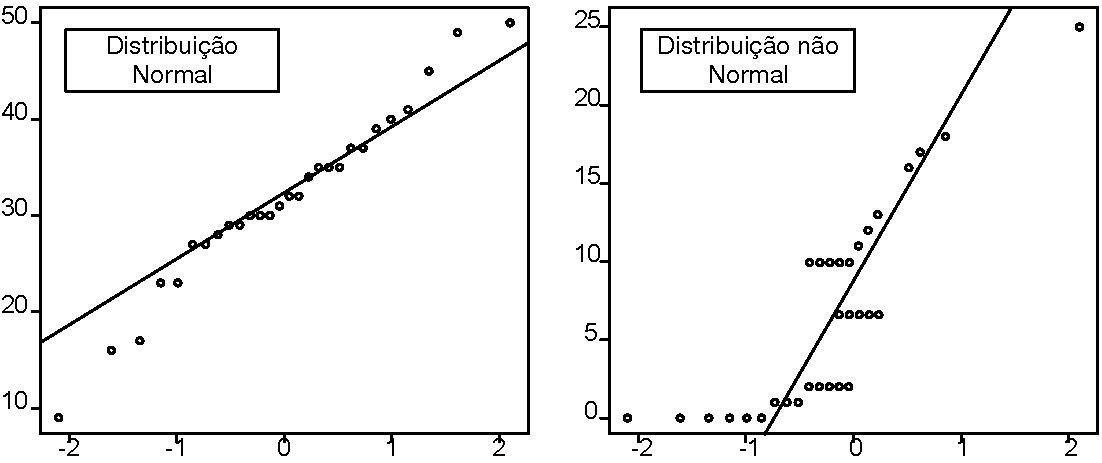
\includegraphics[scale=0.7]{images/qq_plot_exemplo}
	\fautor
\end{figure}

O teste \textbf{Paired T-Test} é utilizado para confrontar dois conjuntos de dados. Esse teste pode ser aplicado somente quando ambos os conjuntos de dados seguirem uma distribuição normal. Se o p-valor (resultado) do \textbf{Paired T-Test} for menor que 0.05 significa que a chance dos dois conjuntos de dados serem estatisticamente semelhantes é menor do que 5\%. Portanto, nesse caso, a hipótese nula deve ser rejeitada~\cite{Wohlin}.

\section{Experimento: Refatorações no contexto do metamodelo KDM}\label{sec:experimento}

Nesta seção, é apresentado um experimento conduzido com o objetivo de analisar as qualidades das refatorações criadas para o metamodelo KDM. Especificamente, a seguinte questão de pesquisa é investida nesse experimento:

\textbf{Questão de Pesquisa 1} (\textbf{$QP_1$}): Como as refatorações criadas para o metamodelo KDM podem ser úteis para engenheiros de software no cenário do mundo real? O benefício esperado de refatoração não está limitada apenas à correção de \textit{bad-smells}, mas também as refatorações podem e devem ser utilizadas para melhorar os atributos de qualidade dos programas, ou seja, melhorar a \aspas{reusabilidade}, \aspas{flexibilidade}, \aspas{facilidade de compreensão} e \aspas{eficácia}.


Dessa forma, para avaliar a \textbf{$QP_1$}, sete sistemas foram escolhidos para aplicar um conjunto de refatorações. Esses sete sistemas são bem conhecidos na literatura e estão implementados na linguagem de programação Java: Xerces-J\footnote{\texttt{http://xerces.apache.org/xerces-j/}}, Jexel\footnote{\texttt{https://jexel.googlecode.com}}, JFreeChart\footnote{\texttt{http://www.jfree.org/jfreechart/}}, Jester\footnote{\texttt{jester.sourceforge.net}}, GanttProject\footnote{\texttt{http://www.ganttproject.biz/}}, ArtofIllusion\footnote{\texttt{www.artofillusion.org}} e JHotDraw\footnote{\texttt{jhotdraw.org}}. Xerces-J é uma família de software para analisar (\textit{parsing}) XML; Jexel é API para escrever expressões regulares em Java; JFreeChart é uma biblioteca Java utilizada para gerar gráficos; Jester é uma biblioteca Java utilizada para gerar teste de unidades; GanttProject é um sistema para gerenciamento de projetos; ArtofIllusion é uma API para modelagem e renderização em 3D; JHotDraw é uma ferramenta para auxiliar a criação de desenhos. Todos esses sistemas foram transformados em instâncias do metamodelo KDM, utilizando a ferramenta MoDisco\footnote{\texttt{https://eclipse.org/MoDisco/}}. 


\begin{table}[h]
\centering
\caption{Sistemas utilizados no Experimento 1.}
\label{tab:sistemas_experimentos}
\begin{tabular}{ | m{2cm} | m{1cm}| m{1cm}| m{1cm} | m{1cm} | } 
\hline
Sistemas & Siglas & Versão & KLOC & Classes \\ 
\hline
Xerces-J & \sigla*{XJ}{Xerces-J} XJ & 2.7.0 & 240 & 991\\ 
\hline
Jexel & \sigla*{JEX}{Jexel} JEX & 1.3 & 50.4 & 75\\
\hline
JFreeChart &\sigla*{JFC}{JFreeChart} JFC & 1.0.9 & 170 & 521\\ 
\hline
Jester & \sigla*{JES}{Jester} JES & 0.7 & 48 & 14\\ 
\hline
GanttProject & \sigla*{GP}{GanttProject} GP & 1.10.2 & 41 & 245\\ 
\hline
ArtofIllusion & \sigla*{AOIL}{ArtofIllusion} AOIL &  2.8.1 & 87 & 459\\ 
\hline
JHotDraw & \sigla*{JHD}{JHotDraw} JHD & 7.0.6 & 16 & 468 \\ 
\hline
\end{tabular}
\end{table}

Na Tabela~\ref{tab:sistemas_experimentos}, é possível visualizar algumas informações sobre os sete sistemas. Como apresentado no Capítulo~\ref{chapter:ferramenta_kdm_re}, a ferramenta KDM-RE apenas auxilia o engenheiro de software a aplicar refatorações em instâncias do metamodelo KDM. É de responsabilidade do engenheiro de software identificar onde aplicar a refatoração, uma vez que a ferramenta KDM-RE ainda não identifica \textit{bad-smells}~\cite{Fowler1999}. Nesse contexto, esses sete sistemas foram aplicados na ferramenta Jdeodorant\footnote{https://marketplace.eclipse.org/content/jdeodorant}, a qual identifica um conjunto de \textit{bad-smells}. Além disso, esses sistemas também foi escolhidos pois na literatura é possível identificar trabalhos que já detectaram e listaram quais são os \textit{bad-smells} de alguns desses sistemas e quais são as possíveis refatorações que devem ser aplicadas como solução~\cite{Kessentini_2011, Ouni_2013, Moha_2010, Kessentini_2010}. %Assim, o engenheiro de software apenas precisa aplicar as refatorações nos sistemas.  



Os \textit{bad-smells} identificados nesses sistemas são: \textit{Blob}/\textit{God Class} (uma classe que faz coisa
demais no sistema), \textit{Data Class} (uma classe demonstra apenas atributos, porém, não os utiliza para realizar nenhum tipo de processamento), \textit{Spaghetti Code} (código com uma estrutura de controle complexo e emaranhado) e \textit{Functional Decomposition} (quando uma classe desempenha uma única função, ao invés de ser um encapsulamento de dados e funcionalidade)~\cite{Fowler1999}. Está fora do escopo deste capítulo se aprofundar nesses \textit{bad-smells}. Porém, uma lista completa dos \textit{bad-smells} identificados nos sete sistemas escolhidos para esse experimento pode ser visualizada nos artigos~\citeonline{Kessentini_2011, Ouni_2013, Moha_2010, Kessentini_2010}.

O principal objetivo desse experimento é verificar se após a aplicação de um conjunto de refatorações com base em \textit{bad-smell} já identificados na literatura~\cite{Kessentini_2011, Ouni_2013, Moha_2010, Kessentini_2010} as refatorações criadas para o metamodelo KDM melhoraram os sistemas em termos de atributos de qualidade. Os atributos de qualidade foram avaliados utilizando o modelo \sigla{QMOOD}{\textit{Quality Model for Object-Oriented Design}}~\cite{Bansiya_QMOOD}. O QMOOD é um modelo de qualidade para POO que estabelece um modelo hierárquico definido e empiricamente validado para avaliar atributos de qualidade de POO. O uso do modelo QMOOD nesse experimento ocorreu, pois: (\textit{i}) o QMOOD é bastante utilizado na literatura~\cite{Keeffe_2008, Seng_2006, Jensen_2010} para avaliar o efeito de refatoração e (\textit{ii}) o QMOOD define seis atributos de qualidade (\aspas{facilidade de compreensão} (\textit{understandability}), \aspas{eficácia} (\textit{effectiveness}), \aspas{extensibilidade} (\textit{extendibility}), \aspas{reusabilidade} (\textit{reusability}), \aspas{funcionalidade} (\textit{functionality}) e \aspas{flexibilidade} (\textit{flexibility})), que são calculados utilizando 11 métricas~\cite{Bansiya_QMOOD} (ver Tabela~\ref{tab:QMOOD_quality_metrics} e Tabela~\ref{tab:QMOOD_quality_metrics2}). 


Nesse experimento apenas quatro atributos de qualidade foram considerados: \aspas{reusabilidade}, \aspas{flexibilidade}, \aspas{facilidade de compreensão} e \aspas{eficácia}. De acordo com~\citeonline{Bansiya_QMOOD} esses atributos podem ser definidos como: 

\begin{itemize}
\item Reusabilidade: Características de POO que permitem um projeto ser reaplicado para um novo problema sem esforço significativo;
\item Flexibilidade: A capacidade de um projeto ser adaptado para disponibilizar novos recursos;
\item Facilidade de Compreensão: Propriedades do projeto que permitem ser facilmente aprendido e compreendido. Está relacionado com a complexidade da estrutura do projeto;
\item Eficácia: Capacidade do projeto obter a funcionalidade e o comportamento desejado, utilizando conceitos e técnicas de POO.
\end{itemize}

O atributo de qualidade \aspas{funcionalidade} foi excluído nesse experimento porque se assume que, por definição, uma refatoração não deve alterar o comportamento/funcionalidade do sistema; em vez disso, apenas altera a estrutura do sistema\footnote{No contexto desta tese, as refatorações criadas preservam a sintaxe e a semântica de instâncias do KDM.}. Também foi excluído o atributo de qualidade denominado \aspas{extensibilidade}, pois, de acordo com~\citeonline{Bansiya_QMOOD}, é um atributo de qualidade subjetivo. 

A Tabela~\ref{tab:QMOOD_quality_metrics} apresenta as propriedades de POO e as métricas que foram utilizadas para mensurar as instâncias do metamodelo KDM antes e após a aplicação das refatorações. A Tabela~\ref{tab:QMOOD_quality_metrics2} apresenta os atributos de qualidade e as propriedades definidas por~\citeonline{Bansiya_QMOOD}. Nesse experimento, o ganho de qualidade é calculado pela comparação de cada atributo de qualidade antes e após a aplicação de um conjunto de refatorações. Com isso, o ganho total da qualidade ($G_{q}$) para cada atributo de qualidade QMOOD pode ser estimado de acordo com a Definição~\ref{def:qmood}.

\begin{definicao}\label{def:qmood}
    \textit{$G_{q_{i}} = q'_{i} - q_{i}$ onde $q'_{i}$ e $q_{i}$ representam os valores do atributo de qualidade $i$ antes e após a aplicação das refatorações, respectivamente.}
\end{definicao}

\begin{table}[!h]
\caption{Métricas utilizadas no modelo QMOOD~\cite{Bansiya_QMOOD}.}
\label{tab:QMOOD_quality_metrics}
\begin{center}
\begin{tabular}{ | m{4cm} | m{4.6cm}| m{6cm} | } 
\hline
Propriedades de Projeto & Métrica & Descrição \\ 
\hline
Tamanho do Projeto & \sigla{DSC}{\textit{Design Size in Classes}} & Número de classes no projeto \\ 
\hline
Hierarquias & \sigla{NOH}{\textit{Number Of Hierarchies}} & Número de Hierarquias \\ 
\hline
Abstração & \sigla{ANA}{\textit{Average Number of Ancestors}} ANA & Média de Ancestrais \\ 
\hline
Encapsulamento & \sigla{DAM}{\textit{Data Access Metric}} & Métrica de acesso a dados \\ 
\hline
Acoplamento & \sigla{DCC}{\textit{Direct Class Coupling}} & Acoplamento direto entre classes \\ 
\hline
Coesão & \sigla{CAM}{\textit{Cohesion Among Methods in class}} & Coesão entre os métodos da classe \\ 
\hline
Composição & \sigla{MOA}{\textit{Measure Of Aggregation}} & Medida de agregação \\ 
\hline
Herança & \sigla{MFA}{\textit{Measure of Functional Abstraction}} & Abstração funcional \\ 
\hline
Polimorfismo & \sigla{NOP}{\textit{Number Of Polymorphic methods}} & Número de métodos polimórficos \\ 
\hline
Troca de Mensagens & \sigla{CIS}{\textit{Class Interface Size}} & Tamanho da interface de uma classe \\ 
\hline
Complexidade & \sigla{NOM}{\textit{Number of methods}} & Quantidade de métodos \\ 
\hline
\end{tabular}
\end{center}
\end{table}

\begin{table}[!h]
\caption{Relacionamento de atributos de qualidade X Propriedade no QMOOD~\cite{Bansiya_QMOOD}.}
\label{tab:QMOOD_quality_metrics2}
\begin{center}
\begin{tabular}{ | m{4cm} | m{10cm} |} 
\hline
Atributo de Qualidade & Fórmula com base nas propriedades de projeto  \\ 
\hline
Reusabilidade & -0,25 x DCC + 0,25 x CAM + 0,5 x CIS + 0,5 x DSC  \\ 
\hline
Flexibilidade & 0.25 x DAM - 0.25 x DCC + 0.5 x MOA +0.5 x NOP \\
\hline
Facilidade de Compreensão & -0.33 x ANA + 0.33 x DAM - 0.33 x DCC + 0.33 x CAM -0.33 x NOP + 0.33 x NOM - 0.33 x DSC \\ 
\hline
Eficácia & 0.2 x ANA + 0.2 x DAM + 0.2 x MOA + 0.2 x MFA + 0.2 x NOP \\ 
\hline
\end{tabular}
\end{center}
\end{table}

\subsection{Definição e Planejamento do Experimento}

Esse experimento foi planejado utilizando o modelo GQM (\textit{Goal, Question, Metric})~\cite{Wohlin}, que é dividido em cinco partes: 

\begin{itemize}
\item \textbf{Objeto de estudo}: o objeto de estudo desse experimento são as refatorações criadas para o metamodelo KDM;
\item \textbf{Propósito}: o propósito desse experimento é avaliar as refatorações criadas para o metamodelo KDM;
\item \textbf{Perspectiva}: esse experimento é executado sobre a perspectiva de um pesquisador;
\item \textbf{Qualidade de foco}: o efeito primário sobre investigação nesse experimento são os atributos de qualidade QMOOD. Mais especificamente, os atributos \aspas{reusabilidade}, \aspas{flexibilidade}, \aspas{facilidade de compreensão} e \aspas{eficácia} após a aplicação de um conjunto de refatoração;
\item \textbf{Contexto}: esse experimento foi conduzido utilizando o ambiente de desenvolvimento Eclipse 4.3.2 em uma máquina 2.5 GHz Intel Core i5 com 8GB de memória física, executando o sistema operacional Mac OS X 10.9.2.
\end{itemize}


O experimento pode ser resumido utilizando o seguinte \textit{template}~\cite{Wohlin}: \textbf{Analisar} as refatorações criadas para o metamodelo KDM; \textbf{com o propósito de} avaliar as refatorações criadas; \textbf{com respeito à} \aspas{reusabilidade}, \aspas{flexibilidade}, \aspas{facilidade de compreensão} e \aspas{eficácia}; \textbf{do ponto de vista dos} pesquisadores; \textbf{no contexto de} distintos sistemas.

\subsubsection{Formulação das Hipóteses}



A \mathbf{$QP_1$} foi formalizada em hipóteses. Para cada atributo de qualidade (\aspas{reusabilidade}, \aspas{flexibilidade}, \aspas{facilidade de compreensão} e \aspas{eficácia}), hipóteses foram criadas como apresentado a seguir:

%\aspas{reusabilidade}, \aspas{flexibilidade}, \aspas{facilidade de compreensão} e \aspas{eficácia}

\begin{itemize}

\item \aspas{Reusabilidade}:

\begin{itemize}
\item \textbf{Hipótese Nula} \textbf{$(H1_{0})$}: Não há diferença significativa entre instâncias do metamodelo KDM antes e após a aplicação de um conjunto de refatorações em relação à reusabilidade. Isso pode ser formalizado como: 

\begin{itemize}
\item $H1_{0}$: $\mu_{reusabilidade_{antes}} = \mu_{reusabilidade_{depois}}$
\end{itemize}

\item \textbf{Hipótese Alternativa} \textbf{$(H1_{1})$}: Há diferença significativa entre as instâncias do metamodelo KDM refatorada e a instância do metamodelo KDM não refatorada em relação à reusabilidade. Isso pode ser formalizado como: 

\begin{itemize}
\item $H1_{1}$: $\mu_{reusabilidade_{antes}} \neq \mu_{reusabilidade_{depois}}$;
\end{itemize}
\end{itemize}

\item \aspas{Flexibilidade}:

\begin{itemize}
%segunda hipotese
\item \textbf{Hipótese Nula} \textbf{$(H2_{0})$}: Não há diferença significativa entre instâncias do metamodelo KDM antes e após a aplicação de um conjunto de refatorações em relação à flexibilidade. Isso pode ser formalizado como: 

\begin{itemize}
\item $H2_{0}$: $\alpha_{flexibilidade_{antes}} = \alpha_{flexibilidade_{depois}}$
\end{itemize}

\item \textbf{Hipótese Alternativa} \textbf{$(H2_{1})$}: Há diferença significativa entre as instâncias do metamodelo KDM refatorada e a instância do metamodelo KDM não refatorada em relação à flexibilidade. Isso pode ser formalizado como: 

\begin{itemize}
\item $H2_{1}$: $\alpha_{flexibilidade_{antes}} \neq \alpha_{flexibilidade_{depois}}$;
\end{itemize}
\end{itemize}

\item \aspas{Facilidade de Compreensão}:

\begin{itemize}
%terceira hipotese
\item \textbf{Hipótese Nula} \textbf{$(H3_{0})$}: Não há diferença significativa entre instâncias do metamodelo KDM antes e após a aplicação de um conjunto de refatorações em relação à facilidade de compreensão. Isso pode ser formalizado como: 

\begin{itemize}
\item $H3_{0}$: $\beta_{compreensao_{antes}} = \beta_{compreensao_{depois}}$
\end{itemize}

\item \textbf{Hipótese Alternativa} \textbf{$(H3_{1})$}: Há diferença significativa entre as instâncias do metamodelo KDM refatorada e a instância do metamodelo KDM não refatorada em relação à facilidade de compreensão. Isso pode ser formalizado como: 

\begin{itemize}
\item $H3_{1}$: $\beta_{compreensao_{antes}} \neq \beta_{compreensao_{depois}}$;
\end{itemize}
\end{itemize}

\item \aspas{Eficácia}:
    
    \begin{itemize}
%terceira hipotese
\item \textbf{Hipótese Nula} \textbf{$(H4_{0})$}: Não há diferença significativa entre instâncias do metamodelo KDM antes e após a aplicação de um conjunto de refatorações em relação à eficácia. Isso pode ser formalizado como: 

\begin{itemize}
\item $H4_{0}$: $\gamma_{eficacia_{antes}} = \gamma_{eficacia_{depois}}$
\end{itemize}

\item \textbf{Hipótese Alternativa} \textbf{$(H4_{1})$}: Há diferença significativa entre as instâncias do metamodelo KDM refatorada e a instância do metamodelo KDM não refatorada em relação à eficacia. Isso pode ser formalizado como: 

\begin{itemize}
\item $H4_{1}$: $\gamma_{eficacia_{antes}} \neq \gamma_{eficacia_{depois}}$;
\end{itemize}
\end{itemize}

\end{itemize}

\subsubsection{Variáveis}

O experimento teve as seguintes variáveis independentes: (\textit{i}) a ferramenta KDM-RE, (\textit{ii}) EMF \textit{Metrics} e Jdeodorant\footnote{https://marketplace.eclipse.org/content/jdeodorant}, (\textit{iii}) o ambiente de desenvolvimento Eclipse versão 4.3.2, (\textit{iv}) a linguagem de programação Java e (\textit{v}) os sete sistemas utilizados (ver Tabela~\ref{tab:sistemas_experimentos}). As variáveis dependentes são as seguintes: (\textit{i}) reusabilidade, (\textit{ii}) flexibilidade, (\textit{iii}) facilidade de compreensão e (\textit{iv}) eficácia.

\subsection{Operação do Experimento}

Depois de definir e planejar o experimento, sua fase de operação foi realizada em duas etapas: Preparação e Execução. Na Figura~\ref{fig:execucao_experimento}, é apresentado o esquema seguido durante a preparação (\ding{182}) e execução (\ding{183}) desse experimento.

\begin{figure}[h]
	\centering
	\caption{Preparação e Execução ilustradas do Experimento 1.}
	\label{fig:execucao_experimento}
	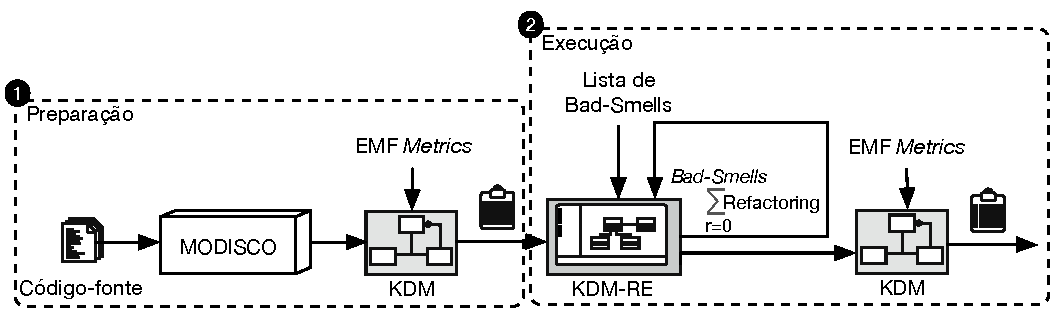
\includegraphics[scale=0.9]{images/Figura_Experimento}
	\fautor
\end{figure}

\subsubsection{Preparação}

Alguns dias antes da realização do experimento, o códigos-fontes dos sete sistemas apresentados na Tabela~\ref{tab:sistemas_experimentos} foram baixados. Posteriormente, todos eles foram transformados em instâncias do metamodelo KDM. Essa transformação foi realizada por meio da ferramenta MoDisco\footnote{\texttt{https://eclipse.org/MoDisco/}} (ver Figura~\ref{fig:execucao_experimento} \ding{182}). Em seguida, para cada instância do metamodelo KDM gerada (que representa os sete sistemas), a ferramenta EMF \textit{Metrics}~\cite{Arendt_2012, Thorsten_2010_durelli} foi executada. Essa ferramenta foi escolhida para mensurar os atributos de qualidade QMOOD (reusabilidade, flexibilidade, facilidade de compreensão e eficácia). Segundo~\citeonline{Arendt_2012, Thorsten_2010_durelli} EMF \textit{Metrics} é um Eclipse \textit{plug-in} que provê a especificação e calcula métricas para qualquer instância de metamodelo que utilize como base o metamodelo EMF, nesse caso, o metamodelo KDM. Mais especificamente, EMF \textit{Metrics} calcula as métricas apresentadas na Tabela~\ref{tab:QMOOD_quality_metrics} e, em seguida, as fórmulas apresentadas na Tabela~\ref{tab:QMOOD_quality_metrics2} foram mensuradas. Como resultado da aplicação do EMF \textit{Metrics} e da Tabela~\ref{tab:QMOOD_quality_metrics2}, uma lista especificando os atributos de qualidade QMOOD (\aspas{reusabilidade}, \aspas{flexibilidade}, \aspas{facilidade de compreensão} e \aspas{eficácia}) foi obtida para os sete sistemas.

\subsubsection{Execução}

Após gerar as instâncias do KDM dos sete sistemas e aplicar a ferramenta EMF \textit{Metrics} para mensurar os atributos de qualidade QMOOD, o próximo passo é a aplicação das refatorações no metamodelo KDM por meio da ferramenta KDM-RE (ver Capítulo~\ref{chapter:ferramenta_kdm_re}). Como já salientado, a ferramenta KDM-RE no seu estado atual não identifica \textit{bad-smells}. Dessa forma, artigos foram lidos na íntegra, pois listam e descrevem \textit{bad-smells} dos sete sistemas escolhidos para esse experimento~\cite{Kessentini_2011, Ouni_2013, Moha_2010, Kessentini_2010}. Esses artigos apresentam uma lista completa dos \textit{bad-smells} identificados, a qual foi utilizada nesse experimento para guiar o engenheiro de software a identificar e escolher qual refatoração aplicar (ver Figura~\ref{fig:execucao_experimento} \ding{183}).

Após tomar conhecimento dos \textit{bad-smells} de cada sistema, refatorações foram escolhidas e depois executadas por meio da ferramenta KDM-RE. Cada refatoração foi aplicada para tentar resolver e remover os \textit{bad-smells} identificados e melhorar, assim, os atributos de qualidade QMOOD. As refatorações escolhidas para remover os \textit{bad-smells} e melhorar os atributos de qualidade foram criteriosamente identificadas no catálogo de refatoração proposto por~\citeonline{Fowler1999}, que descreve qual(is) refatoração(ões) aplicar para resolver um determinado \textit{bad-smell}. 

É importante salientar que as refatorações não foram aplicadas no diagrama de classe, ou seja, não foram aplicadas de forma totalmente manual e por intervenção de \textit{Wizards}, como apresentado no Capítulo~\ref{chapter:ferramenta_kdm_re}. As refatorações não foram executadas manualmente pelo engenheiro de software, uma vez que muitas refatorações foram aplicadas, o que iria demandar muito esforço e tempo para a condução do experimento. Dessa forma, foi criado um arquivo com as refatorações, os parâmetros e os caminhos para cada instância do KDM, que representava os sete sistemas utilizados no experimento. Esse arquivo foi criado tendo como base os \textit{bad-smell} identificados, assim, soube-se previamente qual refatoração aplicar, bem como seus parâmetros – portanto, a ferramenta KDM-RE executou as refatorações de forma semiautomática, diminuindo o tempo para a condução do experimento. Para cada refatoração, um limite de tempo de 5 minutos foi definido, e esse limite de tempo é importante para verificar se a ferramenta KDM-RE não entrou em \textit{loop} infinito.
As refatorações que foram aplicadas nos sete sistemas estão apresentadas na Tabela~\ref{tab:experimento_refatoracoes_aplicadas}, bem como suas respectivas siglas. 



\begin{table}[h]
\centering
\caption{Refatorações aplicadas no experimento 1.}
\label{tab:experimento_refatoracoes_aplicadas}
\begin{tabular}{ | m{3.5cm} | m{1.2cm}|m{2.2cm}| m{1.2cm}|}
\hline
\multicolumn{1}{|c|}{Refatorações} & \multicolumn{1}{c|}{Siglas} & \multicolumn{1}{c|}{Sistemas} & \multicolumn{1}{c|}{Siglas}\\ 
\hline
\multicolumn{1}{|c|}{Move Method} & \multicolumn{1}{c|}{\sigla*{MM}{\textit{Move Method}}MM} & \multicolumn{1}{c|}{Xerces-J} & \multicolumn{1}{c|}{XJ}\\ 
\hline
\multicolumn{1}{|c|}{Move Field} & \multicolumn{1}{c|}{\sigla*{MF}{\textit{Move Field}}MF} & \multicolumn{1}{c|}{Jexel} & \multicolumn{1}{c|}{JEX}\\ 
\hline
\multicolumn{1}{|c|}{Extract Class} & \multicolumn{1}{c|}{\sigla*{EC}{\textit{Extract Class}}EC} & \multicolumn{1}{c|}{JFreeChart} & \multicolumn{1}{c|}{JFC}\\ 
\hline
\multicolumn{1}{|c|}{Extract Interface} & \multicolumn{1}{c|}{\sigla*{EI}{\textit{Extract Interface}}EI} & \multicolumn{1}{c|}{Jester} & \multicolumn{1}{c|}{JES} \\ 
\hline
\multicolumn{1}{|c|}{Move Class} & \multicolumn{1}{c|}{\sigla*{MC}{\textit{Move Class}}MC} & \multicolumn{1}{c|}{GanttProject} & \multicolumn{1}{c|}{GP} \\ 
\hline
\multicolumn{1}{|c|}{Pull Up Field} & \multicolumn{1}{c|}{\sigla*{PUF}{\textit{Pull Up Field}}PUF} & \multicolumn{1}{c|}{ArtofIllusion} & \multicolumn{1}{c|}{AOIL} \\ 
\hline
\multicolumn{1}{|c|}{Pull Up Method} & \multicolumn{1}{c|}{\sigla*{PUM}{\textit{Pull Up Method}}PUM} & \multicolumn{1}{c|}{JHotDraw} & \multicolumn{1}{c|}{JHD} \\ 
\hline
\multicolumn{1}{|c|}{Push Down Field} & \multicolumn{1}{c|}{\sigla*{PDF}{\textit{Push Down Field}}PDF} &\multicolumn{1}{c|}{\textemdash} &\multicolumn{1}{c|}{\textemdash} \\ 
\hline
\multicolumn{1}{|c|}{Push Down Method} & \multicolumn{1}{c|}{\sigla*{PDM}{\textit{Push Down Method}}PDM} &\multicolumn{1}{c|}{\textemdash} &\multicolumn{1}{c|}{\textemdash} \\ 
\hline
\end{tabular}
\end{table}


Na Tabela~\ref{tab:experimento_dados_refatoracoes_aplicadas} é possível observar os dados relacionados com a quantidade de refatorações aplicada em cada sistema. Nota-se que a refatoração \texttt{Move Method} foi a refatoração mais executada, aproximadamente 26.35\%.  Em seguida, a refatoração \texttt{Move Field} foi a segunda refatoração mais aplicada, aproximadamente 13.42\%. A maioria das refatorações aplicadas está relacionada com mover (\texttt{Move Field} e \texttt{Move Method}) e extrair elementos (\texttt{Extract Class}); somando as refatorações \texttt{Move Method}, \texttt{Move Field} e \texttt{Extract Class} têm-se 51.06\% das refatorações aplicadas, ou seja, mais da metade das refatorações. Esses dados estão diretamente relacionados aos \textit{bad-smells} utilizados nesse experimento: \textit{blob}, \textit{data class} e \textit{spaghetti code}. Por exemplo, para remover o \textit{bad-smell} do tipo \textit{blob} é necessário mover elementos de uma classe para outra classe, a fim de reduzir o número de funcionalidades e adicionar comportamento em outras classes. Similarmente, para remover o \textit{bad-smell} do tipo \textit{data class}, deve-se aplicar a refatoração \texttt{Move Method}. Ainda observando a Tabela~\ref{tab:experimento_dados_refatoracoes_aplicadas}, é possível notar que as refatorações menos aplicadas foram: \texttt{Push Up Method}, \texttt{Push Up Field} e \texttt{Move Class}, respectivamente. 

\begin{table}[h]
\centering
\caption{Quantidade de refatorações aplicadas no experimento 1.}
\label{tab:experimento_dados_refatoracoes_aplicadas}
\begin{tabular}{c|c|c|c|c|c|c|c|c|c|}
\cline{2-10}
                                   & \multicolumn{9}{c|}{Sistemas}                                \\ \hline
\multicolumn{1}{|c|}{Refatorações} & XJ & JEX & JFC & JES & GP & AOIL & JHD & Média & Porcentagem \\ \hline
\multicolumn{1}{|c|}{MM}           & 40 & 30  & 45  & 35  & 43 & 45   & 23  & 37.29 & 26.34\%     \\ \hline
\multicolumn{1}{|c|}{MF}           & 25 & 15  & 20  & 16  & 21 & 23   & 13  & 19.00 & 13.42\%     \\ \hline
\multicolumn{1}{|c|}{EC}           & 15 & 20  & 20  & 19  & 12 & 15   & 11  & 16.00 & 11.30\%     \\ \hline
\multicolumn{1}{|c|}{EI}           & 13 & 10  & 15  & 16  & 8  & 12   & 10  & 12.00 & 8.48\%      \\ \hline
\multicolumn{1}{|c|}{MC}           & 9  & 11  & 7   & 13  & 10 & 10   & 18  & 11.14 & 7.87\%      \\ \hline
\multicolumn{1}{|c|}{PUF}          & 12 & 14  & 5   & 8   & 12 & 11   & 9   & 10.14 & 7.16\%      \\ \hline
\multicolumn{1}{|c|}{PUM}          & 10 & 9   & 8   & 6   & 8  & 14   & 13  & 9.71  & 6.86\%     \\ \hline
\multicolumn{1}{|c|}{PDF}          & 17 & 13  & 15  & 10  & 9  & 16   & 8   & 12.57 & 8.88\%      \\ \hline
\multicolumn{1}{|c|}{PDM}          & 16 & 12  & 14  & 11  & 10 & 18   & 15  & 13.71 & 9.69\%      \\ \hline
\multicolumn{1}{|c|}{TOTAL}          & 157
 & 134 & 149 & 134  & 133 & 164   & 120  & \textemdash & 100.00\%      \\ \hline
\end{tabular}
\end{table}


Após a aplicação das refatorações nos sete sistemas, a ferramenta EMF \textit{Metrics} foi executada novamente para mensurar os atributos de qualidade QMOOD. A análise dos dados é apresentada na próxima seção.

\subsection{Análise dos Dados do Experimento}

Na Tabela~\ref{tab:dados_coletados_experimento_1}, é possível observar os dados relacionados aos atributos (reusabilidade, flexibilidade, facilidade de compreensão e eficácia) de qualidade avaliados no experimento 1 antes e após a aplicação das refatorações apresentadas na Tabela~\ref{tab:experimento_dados_refatoracoes_aplicadas}. A Tabela~\ref{tab:dados_coletados_experimento_1} possui sete colunas; a coluna denominada \aspas{Antes} representa as métricas mensuradas dos sistemas antes de aplicar as refatorações. A coluna \aspas{Depois} representa as métricas coletadas dos sistemas após a aplicação das refatorações e a coluna \aspas{Diferença} representa a discrepância das colunas \aspas{Antes} e \aspas{Depois}, ou seja, a diferença entre as métricas é calculada da seguinte forma: \aspas{Depois}-\aspas{Antes}. Os mesmos dados são plotados nos gráficos de barra mostrados na Figura~\ref{fig:barchartRefactoringBeforeAndAfter}. 


\begin{table}[h]
\centering
\caption{Dados coletados do experimento 1.}
\label{tab:dados_coletados_experimento_1}
\begin{tabular}{c|l|l|l|l|l|l|}
\cline{2-7}
\multicolumn{1}{l|}{}               & \multicolumn{3}{c|}{Reusabilidade}             & \multicolumn{3}{c|}{Flexibilidade} \\ \hline
\multicolumn{1}{|c|}{Sistemas}      & Antes         & Depois        & Diferença      & Antes     & Depois    & Diferença  \\ \hline
\multicolumn{1}{|c|}{Xerces-J}      & \multicolumn{1}{c|}{0.061}          & \multicolumn{1}{c|}{0.082}          & \multicolumn{1}{c|}{0.021} & \multicolumn{1}{c|}{0.128}      & \multicolumn{1}{c|}{0.136}      &\multicolumn{1}{c|}{0.008}\\ \hline
\multicolumn{1}{|c|}{Jexel}         & \multicolumn{1}{c|}{0.112}& \multicolumn{1}{c|}{0.124} & \multicolumn{1}{c|}{0.012} & \multicolumn{1}{c|}{0.145}      & \multicolumn{1}{c|}{0.152}      &\multicolumn{1}{c|}{0.007}\\ \hline
\multicolumn{1}{|c|}{JFreeChart}    & \multicolumn{1}{c|}{0.147}& \multicolumn{1}{c|}{0.161}& \multicolumn{1}{c|}{0.014} & \multicolumn{1}{c|}{0.129}      & \multicolumn{1}{c|}{0.143}      & \multicolumn{1}{c|}{0.014} \\ \hline
\multicolumn{1}{|c|}{Jester}        & \multicolumn{1}{c|}{0.072}& \multicolumn{1}{c|}{0.068}& \multicolumn{1}{c|}{-0.004} & \multicolumn{1}{c|}{0.081}      & \multicolumn{1}{c|}{0.094}      & \multicolumn{1}{c|}{0.013}  \\ \hline
\multicolumn{1}{|c|}{GanttProject}  & \multicolumn{1}{c|}{0.089}& \multicolumn{1}{c|}{0.127}          & \multicolumn{1}{c|}{0.038} & \multicolumn{1}{c|}{0.153}      & \multicolumn{1}{c|}{0.178}      &  \multicolumn{1}{c|}{0.025} \\ \hline
\multicolumn{1}{|c|}{ArtofIllusion} & \multicolumn{1}{c|}{0.041}          & \multicolumn{1}{c|}{0.092}          & \multicolumn{1}{c|}{0.051} & \multicolumn{1}{c|}{0.111}      & \multicolumn{1}{c|}{0.136}      & \multicolumn{1}{c|}{0.025} \\ \hline
\multicolumn{1}{|c|}{JHotDraw}      & \multicolumn{1}{c|}{0.028}          & \multicolumn{1}{c|}{0.057}          & \multicolumn{1}{c|}{0.029} & \multicolumn{1}{c|}{0.039}      & \multicolumn{1}{c|}{0.054}      & \multicolumn{1}{c|}{0.015}\\ \hline
\multicolumn{1}{|c|}{Média}         & \multicolumn{1}{c|}{0.078}         & \multicolumn{1}{c|}{0.094}         & \multicolumn{1}{c|}{0.023} & \multicolumn{1}{c|}{0.112}     & \multicolumn{1}{c|}{0.127}     & \multicolumn{1}{c|}{0.015} \\ \hline
\multicolumn{1}{|l|}{Porcentagem}   & 43.62\%       & 56.38\%       &\multicolumn{1}{c|}{12.77\%}                & 46.81\%   & 53.19\%   & \multicolumn{1}{c|}{6.37\%}\\ \hline
                                    & \multicolumn{3}{c|}{Facilidade de Compreensão} & \multicolumn{3}{c|}{Eficácia}      \\ \hline
\multicolumn{1}{|c|}{Sistemas}      & Antes         & Depois        & Diferença      & Antes     & Depois    & Diferença  \\ \hline
\multicolumn{1}{|c|}{Xerces-J}      & \multicolumn{1}{c|}{-0.21}& \multicolumn{1}{c|}{-0.289}          &\multicolumn{1}{c|}{-0.079}&\multicolumn{1}{c|}{0.071}&\multicolumn{1}{c|}{0.082}&\multicolumn{1}{c|}{0.011}            \\ \hline
\multicolumn{1}{|c|}{Jexel}         & \multicolumn{1}{c|}{-0.162}          & \multicolumn{1}{c|}{-0.218}          &\multicolumn{1}{c|}{-0.056} & \multicolumn{1}{c|}{0.052}          & \multicolumn{1}{c|}{0.061}          &\multicolumn{1}{c|}{0.009}            \\ \hline
\multicolumn{1}{|c|}{JFreeChart}    & \multicolumn{1}{c|}{-0.159}          & \multicolumn{1}{c|}{-0.213} &\multicolumn{1}{c|}{-0.054}&\multicolumn{1}{c|}{0.04}&\multicolumn{1}{c|}{0.031}&\multicolumn{1}{c|}{-0.009}\\ \hline
\multicolumn{1}{|c|}{Jester}        & \multicolumn{1}{c|}{-0.143}          & \multicolumn{1}{c|}{-0.236}          &\multicolumn{1}{c|}{-0.093}&\multicolumn{1}{c|}{0.097}&\multicolumn{1}{c|}{0.092}&\multicolumn{1}{c|}{-0.005}\\ \hline
\multicolumn{1}{|c|}{GanttProject}  & \multicolumn{1}{c|}{-0.231}          & \multicolumn{1}{c|}{-0.289}          &\multicolumn{1}{c|}{-0.058}&\multicolumn{1}{c|}{0.046}&\multicolumn{1}{c|}{0.057}&\multicolumn{1}{c|}{0.011}\\ \hline
\multicolumn{1}{|c|}{ArtofIllusion} & \multicolumn{1}{c|}{-0.093}          & \multicolumn{1}{c|}{-0.147}          &\multicolumn{1}{c|}{-0.054}&\multicolumn{1}{c|}{0.032}&\multicolumn{1}{c|}{0.043}&\multicolumn{1}{c|}{0.012}\\ \hline
\multicolumn{1}{|c|}{JHotDraw}             & \multicolumn{1}{c|}{-0.042}          & \multicolumn{1}{c|}{-0.098}          &\multicolumn{1}{c|}{-0.054}&\multicolumn{1}{c|}{0.011}&\multicolumn{1}{c|}{0.022}&\multicolumn{1}{c|}{0.011}\\ \hline
\multicolumn{1}{|c|}{Média}         & \multicolumn{1}{c|}{-0.148}         & \multicolumn{1}{c|}{-0.212}         &\multicolumn{1}{c|}{-0.064}&\multicolumn{1}{c|}{0.049}&\multicolumn{1}{c|}{0.055}&\multicolumn{1}{c|}{0.005}\\ \hline
\multicolumn{1}{|l|}{Porcentagem}   & 41.11\%       & 58.89\%       &\multicolumn{1}{c|}{17.79\%}&  \multicolumn{1}{c|}{47.35\%}  &  \multicolumn{1}{c|}{52.65\%}  &\multicolumn{1}{c|}{5.29\%}\\ \hline
\end{tabular}
\end{table}

Nota-se que todos os atributos de qualidade foram melhorados após a aplicação das refatorações: (\textit{i}) \aspas{reusabilidade} (antes = 43.62\%, depois = 56.38\% e diferença = 12.77\%), \aspas{flexibilidade} (antes = 46.81\%, depois = 53.19\% e diferença = 6.37\%), \aspas{facilidade de compreensão} (antes = 41.11\%, depois = 58.89\% e diferença = 17.79\%) e \aspas{eficácia} (antes = 47.35\%, depois = 52.65\% e diferença = 5.29\%).
É importante observar que o atributo de qualidade \aspas{facilidade de compreensão} foi o que alcançou o maior ganho, aproximadamente 59\%. Por outro lado, o atributo de qualidade \aspas{eficácia} teve o menor ganho, alcançando  52.65\%. Isso deve-se principalmente às refatorações aplicadas. Por exemplo, a maioria das refatorações aplicadas (\texttt{Move Method}, \texttt{Move Field} e \texttt{Extract Class} (ver Tabela~\ref{tab:experimento_dados_refatoracoes_aplicadas})) aumenta o acoplamento (DCC), coesão (CAM) e tamanho do projeto (DSC), que são métricas utilizadas para calcular o atributo de qualidade Facilidade de Compreensão.

Além disso, pode-se também observar na Figura~\ref{fig:barchartRefactoringBeforeAndAfter} que o sistema JHotDraw produziu o menor aumento para os quatro atributos de qualidade. Acredita-se que a principal razão disso é que JHotDraw é conhecido na literatura por seguir as melhores práticas de projeto e implementação~\cite{Kessentini_2010}, assim, poucas refatorações precisaram ser aplicadas nesse sistema.


\begin{figure}[h]
	\centering
	\caption{Gráficos resultantes antes e após as refatorações.}
	\label{fig:barchartRefactoringBeforeAndAfter}
	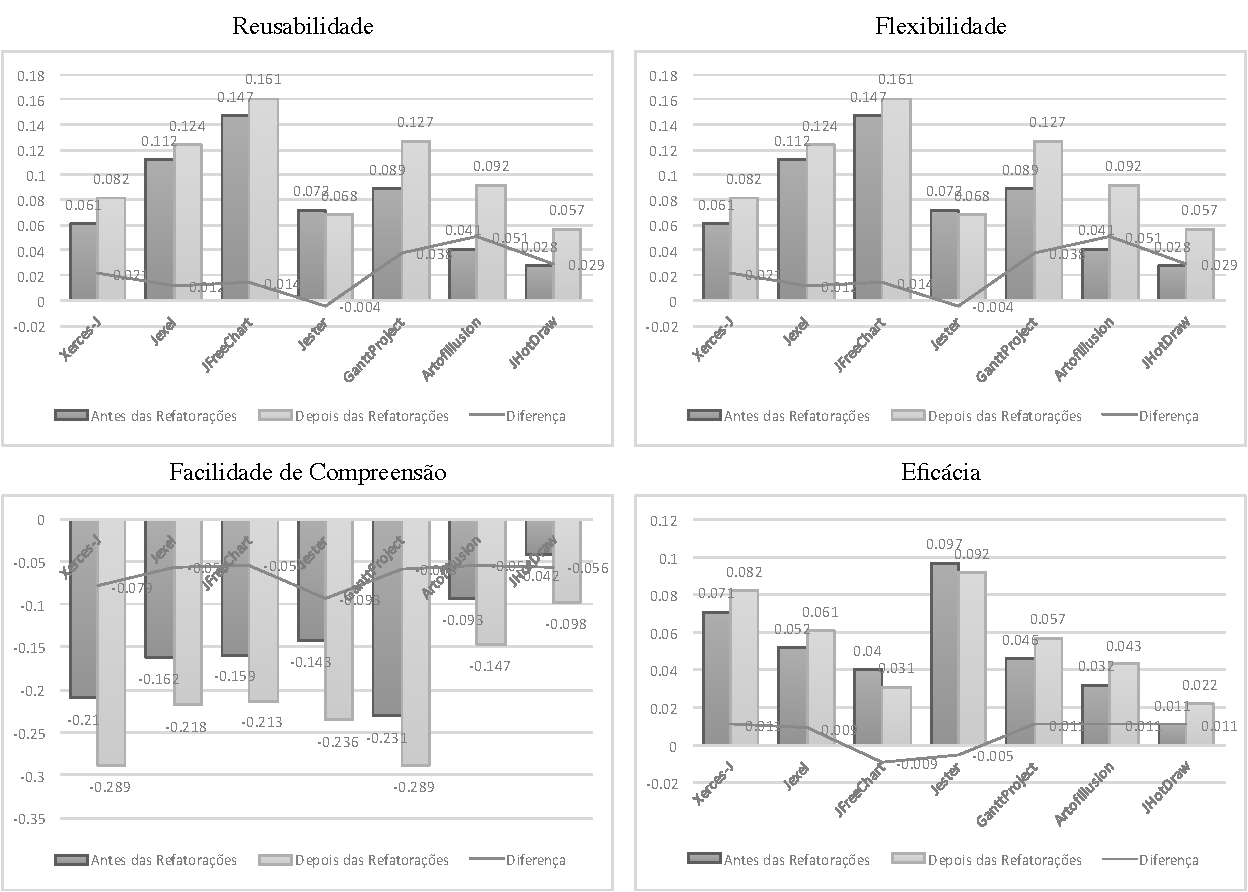
\includegraphics[scale=0.7]{images/GraficoDeBarraTodasDia140116}
	\fautor
\end{figure}


%\begin{figure}[!h]    
%\begin{minipage}[h]{0.5\textwidth}
%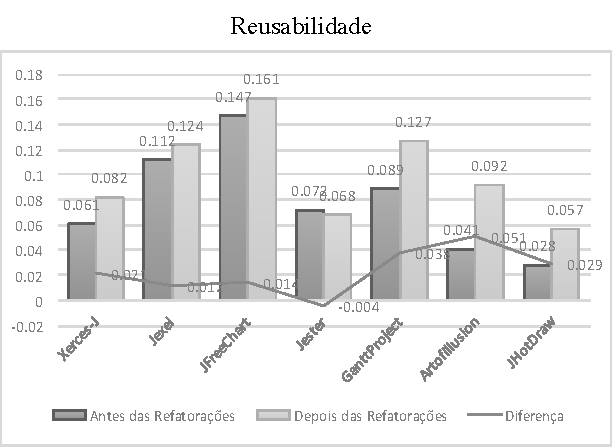
\includegraphics[width=\linewidth]{images/GraficoBarraExperimentoReusabilidadeNovo}
%\caption{Reusabilidade antes e depois das refatorações.}
%\label{fig:immediate}
%\end{minipage}
%\hspace{\fill}
%\begin{minipage}[h]{0.5\textwidth}
%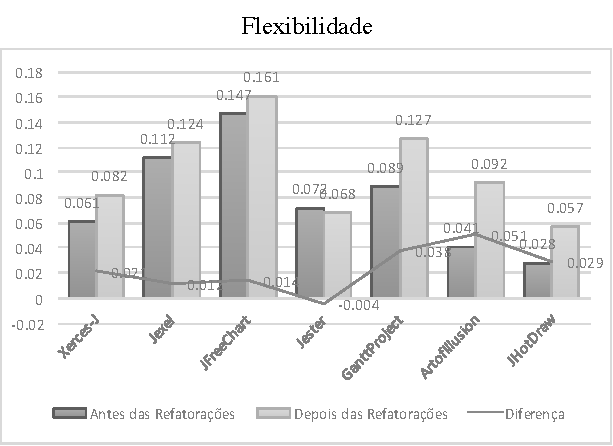
\includegraphics[width=\linewidth]{images/GraficoBarraExperimentoFlexibilidadeNovo}
%\caption{Flexibilidade antes e depois das refatorações.}
%\label{fig:proximal}
%\end{minipage}

%\vspace*{0.5cm} % (or whatever vertical separation you prefer)
%\begin{minipage}[h]{0.5\textwidth}
%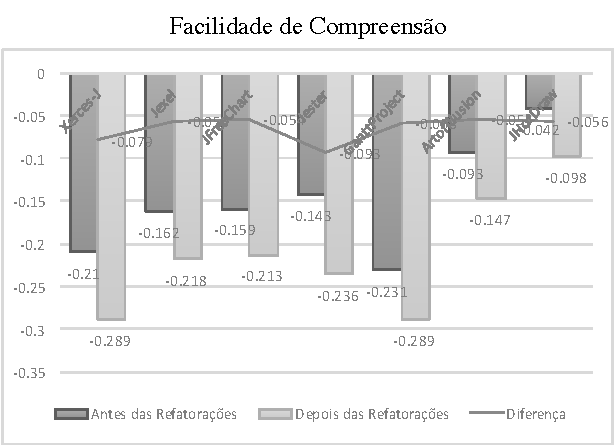
\includegraphics[width=\linewidth]{images/GraficoBarraExperimentoFacilidadeDeCompreensaoNovo}
%\caption{Facilidade de Compreensão antes e depois das refatorações.}
%\label{fig:distal}
%\end{minipage}
%\hspace{\fill}
%\begin{minipage}[h]{0.5\textwidth}
%\includegraphics[width=\linewidth]{images/GraficoBarraExperimen%toEficaciaNovo}
%\caption{Eficácia antes e depois das refatorações.}
%\label{fig:combined}
%\end{minipage}

%\end{figure}

\begin{figure}[h]
	\centering
	\caption{Gráficos resultantes do teste de normalidade.}
	\label{fig:qq_plot_experimento1}
	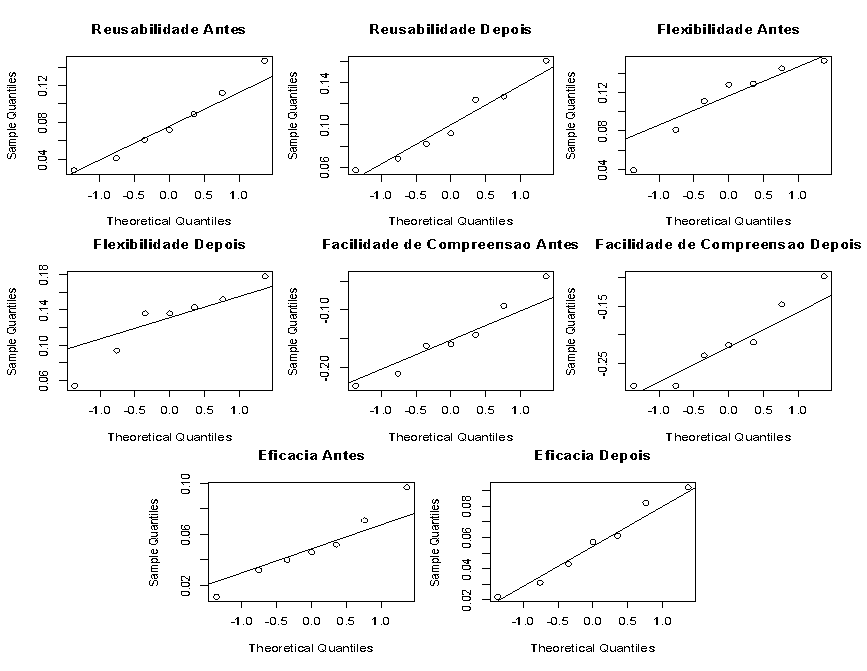
\includegraphics[scale=0.9]{images/QQPlotDia140116}
	\fautor
\end{figure}

\subsubsection{Teste das Hipóteses}

Nesta seção, são apresentados os resultados dos testes estatísticos aplicados sobre os dados coletados no experimento. Antes de aplicar qualquer teste estatístico, é importante verificar se um conjunto de dados segue, ou não, uma distribuição normal (ver Seção~\ref{sec:shapiro_wilk}). Dessa forma, para os conjuntos de dados (antes e depois das refatorações) dos atributos de qualidade \aspas{reusabilidade}, \aspas{flexibilidade}, \aspas{facilidade de compreensão} e \aspas{eficácia}s apresentados na Tabela~\ref{tab:dados_coletados_experimento_1}, aplicou-se o teste \textbf{Shapiro-Wilk} para verificar se os dados seguem uma distribuição normal. Além disso, para cada conjunto de dados também foram criados gráficos de probabilidade denominados \textit{Q-Q Plot}, ver Figura~\ref{fig:qq_plot_experimento1}. Como pode ser observado na Tabela~\ref{tab:dados_coletados_experimento_1}, o p-valor resultante para cada atributo de qualidade é: reusabilidade (antes = 0.8988, depois = 0.7245), flexibilidade (antes = 0.3298, depois = 0.416), facilidade de compreensão (antes = 0.8137, depois = 0.4716) e eficácia (antes = 0.9355, depois = 0.8362). É visto que todos os p-valor dos testes foram superior a 0.05, então, pode-se afirmar, com nível de confiança de 95\%, que os dados seguem uma distribuição normal. Isso também pode ser verificado nos gráficos mostrados na Figura~\ref{fig:qq_plot_experimento1}. Nota-se que em tais gráficos os pontos estão formados pelo quantis amostrais e o pontos alinham-se nas respectivas retas, com isso, pode-se afirmar que os dados estão normalizados.

\begin{table}[h]
\centering
\caption{\textit{Shapiro-Wilk} aplicado para verificar se os dados seguem uma distribuição normal.}
\label{tab:shapiro_experimento_1}
\begin{tabular}{|c|c|c|c|}
\hline
\multicolumn{4}{|c|}{Reusabilidade}                       \\ \hline
\multicolumn{2}{|c|}{Antes} & \multicolumn{2}{c|}{Depois} \\ \hline
w=0.97        & p-valor=0.8988        & w=0.9494        & p-valor=0.7245        \\ \hline
\multicolumn{4}{|c|}{Flexibilidade}                       \\ \hline
\multicolumn{2}{|c|}{Antes} & \multicolumn{2}{c|}{Depois} \\ \hline
w=0.8998        & p-valor=0.3298        & w=0.9129        & p-valor=0.416        \\ \hline
\multicolumn{4}{|c|}{Facilidade de Compreensão}           \\ \hline
\multicolumn{2}{|c|}{Antes} & \multicolumn{2}{c|}{Depois} \\ \hline
w=0.9594        & p-valor=0.8137        & w=0.9203        & p-valor=0.4716         \\ \hline
\multicolumn{4}{|c|}{Eficácia}                            \\ \hline
\multicolumn{2}{|c|}{Antes} & \multicolumn{2}{c|}{Depois} \\ \hline
w=0.9756        & p-valor=0.9355         & w=0.9621        & p-valor=0.8362        \\ \hline
\end{tabular}
\end{table}

Como os dados estão normalizados (ver Tabela~\ref{tab:shapiro_experimento_1}), o \textit{Paried T-Test} foi aplicado sobre os dados para verificar as hipóteses da \mathbf{$QP_1$} do experimento (Seção~\ref{sec:experimento}). Como mostrado na Tabela~\ref{tab:experimento_1_10_15}, todos atributos de qualidade foram p-valor < 0.05; então, com nível de confiança de 95\%, existem evidências de diferença entre os atributos de qualificação antes e após a aplicação das refatorações. Portanto, podem-se refutar as hipóteses nulas \textbf{$H1_{0}$}, \textbf{$H2_{0}$} e \textbf{$H3_{0}$} e as hipóteses alternativas foram aceitas. O atributo de qualidade \aspas{eficácia} tem uma relação com o atributo de qualidade \aspas{facilidade de compreensão}, pois quando um é melhorado o outro tende a piorar. Dessa maneira, para o atributo de qualidade \aspas{eficácia} não se pode refutar a hipótese nula, porque os dados não se demostraram estatisticamente significantes para refutá-la, ou seja, não houve evidência suficientemente forte para provar que a hipótese nula era falsa.


\begin{table}[]
\centering
\caption{\textit{Paried T-Test} aplicado sobre os dados para verificar as hipóteses da \mathbf{$QP_1$}.}
\label{tab:experimento_1_10_15}
\begin{tabular}{|m{1cm}|l|l|m{7.1cm}|}
\hline
\multicolumn{1}{|c|}{Atributo de Qualidade} & \multicolumn{1}{c|}{T} & \multicolumn{1}{c|}{P-valor} & \multicolumn{1}{c|}{Comentário} \\ \hline
\multicolumn{1}{|c|}{Reusabilidade} & \multicolumn{1}{c|}{-3.3498} & \multicolumn{1}{c|}{0.01542} & Refuta-se \textbf{$(H1_{0})$} com significância de 5\%\\ \hline
\multicolumn{1}{|c|}{Flexibilidade} &\multicolumn{1}{c|}{-5.5602}& \multicolumn{1}{c|}{0.001433} &Refuta-se \textbf{$(H2_{0})$} com significância de 5\%\\ \hline
\multicolumn{1}{|c|}{Facilidade de Compreensão} & \multicolumn{1}{c|}{11.0194} &    \multicolumn{1}{c|}{3.322e-05}&Refuta-se \textbf{$(H3_{0})$} com significância de 5\%\\ \hline
\multicolumn{1}{|c|}{Eficácia}&\multicolumn{1}{c|}{-1.6951}&\multicolumn{1}{c|}{0.141}&\multicolumn{1}{c|}{Não se refuta \textbf{$(H4_{0})$}, pois 0.141 > 0.05}\\ \hline
\end{tabular}
\end{table}

\subsection{Ameaças à Validade do Experimento}
São apresentados, aqui,  os itens que podem afetar os valores e a conclusão do experimento 1. O experimento 1 é afetado pelas ameaças à validade listadas abaixo.

\textbf{Validade Externa:} refere-se à generalidade do experimento. O experimento 1, foi conduzido em sete sistemas diferentes de código aberto amplamente utilizados, pertencentes a diferentes domínios e com tamanhos diferentes. No entanto, não é possível afirmar que os resultados podem ser generalizados para todas as aplicações Java instanciadas para o metamodelo KDM, bem como para outras linguagens de programação, e outros engenheiros de software. Outra ameaça pode ser o número limitado de sujeitos/sistemas estudados, o que ameaça externamente a generalização dos resultados do presente trabalho. Replicações futuras desse estudo são necessárias para confirmar o resultado da abordagem.


\textbf{Validade por Construção}: está preocupada com a relação entre a teoria e o que é observado. Como a ferramenta KDM-RE no seu estado atual não identifica \textit{bad-smells}, a escolha das refatorações aplicadas está totalmente dependente do conhecimento de terceiros. Dessa forma, para mitigar essa ameaça, os sete sistemas foram escolhidos, pois outros pesquisadores já haviam identificado e listado os \textit{bad-smells} na literatura~\cite{Kessentini_2011, Ouni_2013, Moha_2010, Kessentini_2010}.

\textbf{Validade de Conclusão}: está relacionada com a precisão das métricas empregadas durante o experimento 1. Para mitigar essa ameaça, utilizaram-se métricas já consolidadas na literatura, tais como QMOOD. 

\section{Considerações Finais}\label{sec:consideracoes_finais_experimento}

Neste capítulo foi apresentado o experimento realizado para avaliar as refatorações criadas para o metamodelo KDM. Esse experimento foi previamente planejado com base no objetivo pretendido, nos recursos a serem utilizados e nas variáveis. Além disso, testes estatísticos foram aplicados para obter maior confiabilidade nos resultados obtidos.

Sete sistemas foram utilizados no experimento, os quais foram transformados em instâncias KDM por meio da ferramenta MoDisco. Em seguida, a ferramenta EMF \textit{Metrics} foi usada para mensurar os atributos de qualidade QMOOD. Como já salientado, a ferramenta KDM-RE no seu estado atual não identifica \textit{bad-smells}. Dessa forma, artigos foram lidos na íntegra, pois listam e descrevem \textit{bad-smells} dos sete sistemas escolhidos para esse experimento. Após tomar conhecimento dos \textit{bad-smells} de cada sistema, refatorações foram escolhidas e depois executadas por meio da ferramenta KDM-RE. Note que, as refatorações não foram aplicadas no diagrama de classe, ou seja, não foram aplicadas de forma totalmente manual e por intervenção de \textit{Wizards}, como apresentado no Capítulo~\ref{chapter:ferramenta_kdm_re}. Dessa forma, foi criado um arquivo com as refatorações, os parâmetros e os caminhos para cada instância do KDM, que representava os sete sistemas utilizados no experimento.

A refatoração \texttt{Move Method} foi a refatoração mais executada, aproximadamente 26.35\%.  Em seguida, a refatoração \texttt{Move Field} foi a segunda refatoração mais aplicada, aproximadamente 13.42\%. A maioria das refatorações aplicadas está relacionada com mover (\texttt{Move Field} e \texttt{Move Method}) e extrair elementos (\texttt{Extract Class}); somando as refatorações \texttt{Move Method}, \texttt{Move Field} e \texttt{Extract Class} têm-se 51.06\% das refatorações aplicadas, ou seja, mais da metade das refatorações. Após a aplicação das refatorações nos sete sistemas, a ferramenta EMF \textit{Metrics} foi executada novamente para mensurar os atributos de qualidade QMOOD.

Diante disso, foi visto nos sete sistemas todos os atributos de qualidade foram melhorados após a aplicação das refatorações: (\textit{i}) \aspas{reusabilidade} (antes = 43.62\%, depois = 56.38\% e diferença = 12.77\%), \aspas{flexibilidade} (antes = 46.81\%, depois = 53.19\% e diferença = 6.37\%), \aspas{facilidade de compreensão} (antes = 41.11\%, depois = 58.89\% e diferença = 17.79\%) e \aspas{eficácia} (antes = 47.35\%, depois = 52.65\% e diferença = 5.29\%).
É importante observar que o atributo de qualidade \aspas{facilidade de compreensão} foi o que alcançou o maior ganho, aproximadamente 59\%. Por outro lado, o atributo de qualidade \aspas{eficácia} teve o menor ganho, alcançando  52.65\%. Isso deve-se principalmente às refatorações aplicadas. Por exemplo, a maioria das refatorações aplicadas (\texttt{Move Method}, \texttt{Move Field} e \texttt{Extract Class}) aumenta o acoplamento (DCC), coesão (CAM) e tamanho do projeto (DSC), que são métricas utilizadas para calcular o atributo de qualidade Facilidade de Compreensão.